\begin{doublespace}

In addition to designing a user interface that is easy to use and aesthetically pleasing (as described in Chapter~\ref{sec:design_ui}), the backend code of the application needed its own design. The goal of the backend system was to extend the previous gearbox design software (\cite{holman_automated_2018}) to allow new features to be added (especially a preview window), and to convert the existing Windows Forms codebase to WPF. This section will describe some of the system design decisions made.

\subsection{Design Pattern}

Before writing any code, we needed to determine a design pattern. A design pattern describes the different parts of an application and the relationship between them, while leaving the implementation up to the developer. Microsoft recommends using the \emph{Model-View-ViewModel} (MVVM) architecture with WPF applications (\cite{smith_patterns_2009}).

The MVVM design pattern has three major parts:
\begin{itemize}
    \item Model -- Stores information about the application's state, no UI components
    \item View -- User interface definition
    \item ViewModel -- Handles interactions between the model and the view
\end{itemize}

The Model of the application is represented by data classes --  classes that store data and have methods to perform operations using this data. The Model classes must not have any UI interaction in them by design.

The View of the application is represented by XAML files. These files describe the location and behavior of every UI element. Each window and page is defined in its own XAML file. 

ViewModel elements may be defined inside the XAML files via data binding, but are also defined in a C\# file. When a WPF window is created in code, a XAML (\texttt{.xaml}) file and a C\# (\texttt{.xaml.cs}) file are created. The XAML file is used for storing information about the view, such as placements of controls and event handlers, while the C\# file is used for user interaction and ViewModel code. For example, you can specify a method that runs whenever a user clicks a button. This method can then interact with the Model classes.

In addition to the MVVM design pattern, we also implemented the main Model class (\texttt{GearBoxInfo}) using the singleton design pattern. A singleton object is a single instance of an object that is shared among the entire application. Since the application must only have one \texttt{GearBoxInfo} class (since the user can only have one open at a time), the singleton pattern works perfectly. It simplifies the passing of data between classes since all classes access the same object. This helps reduce data inconsistency and simplifies the programming since the programmer does not need to worry about passing the object to other functions or classes that need it.

The two singleton objects, \texttt{GearBoxInfo} and \texttt{GearBoxSettings} were designed with thread-safety in mind (since these objects may be accessed from different threads). Considering this need, each singleton class is defined as seen in Listing~\ref{lst:singleton}. The lock object defined on line 16 guarantees thread-safety by ensuring that only one thread may access \texttt{Instance} at a time.

\begin{listing}[htbp]
    \inputminted[
        fontsize=\small,
        linenos,
        frame=lines
    ]{csharp}{code/singleton.cs}
    \caption{Singleton object definition of \texttt{GearBoxSettings}.}
    \label{lst:singleton}
\end{listing}

Since \texttt{Instance} is defined as a \texttt{static} variable, it can be accessed from any file in the code by calling \texttt{GearBoxSettings.Instance}. Without using a singleton object, in order to access \texttt{GearBoxSettings}, an instance of this object would need to be passed to every class via a function call. This can cause data integrity issues if the instance is not passed along properly. Using a singleton object simplifies the process and reduces the amount of possible errors significantly. It also makes the code easier to maintain and build upon in the future if needed since the code is more simple.

\subsubsection{Model}

As described before, the Model section of the application are those classes which describe the data of an application without having reference to any user interface components. With respect to our system, this is comprised of classes about gears, gear sets, and shafts. It also contains internal application settings and user settings, as well as a function to export gear data to SolidWorks (SolidWorks API handler). Most of the model was taken directly from the previous gearbox application, with only minor additions or fixes. The model objects will be described below. All values relating to gear sets, gears, and shafts (in the tables below) are defined by the user using the application interface.

The diagram shown in Figure~\ref{fig:uml} also shows the information in the tables, as well as the relationship between all four model classes.

\noindent\textbf{GearBoxInfo} \\
The \texttt{GearBoxInfo} class is the singleton object which represents all the parts of a gearbox. It contains gearsets and shafts, as well as other information specific to the gearbox. See Table~\ref{tab:gearboxinfo} for all the properties in this class.
\begin{table}[htbp]
    \centering
    \caption{\texttt{GearBoxInfo} properties.}
    \label{tab:gearboxinfo}
    \begin{tabularx}{1\textwidth}{||Y|Y|Y||}
    \hline Property & Type & Description \\ \hline \hline
    Name & String & Name of the gearbox the user has open. \\ \hline
    GearSets & List of \texttt{GearSet}& All the gear sets contained in this gearbox \\ \hline
    Shafts & List of \texttt{Shaft} & All the shafts contained in this gearbox \\ \hline
    \end{tabularx}
\end{table}


\noindent\textbf{GearSet} \\
A \texttt{GearSet} is an object which contains the gears of the gearbox. In general, a gear set refers to a set of gears which are touching each other (not on the same shaft). The \texttt{GearSet} class has a list of \texttt{Gear}s, as well as some other properties specific to the gear set such as the material and gear type. See Table~\ref{tab:gearset} for a list of properties and descriptions.

\begin{table}[htbp]
    \centering
    \caption{\texttt{GearSet} properties.}
    \label{tab:gearset}
    \begin{tabularx}{1\textwidth}{||Y|Y|Y||}
    \hline Property & Type & Description \\ \hline \hline
    Name & String & Name of the gear set (generally follows the format ``GearSet $<$number$>$'' e.g. ``GearSet 1''). \\ \hline
    Type & String & The type of the gears in this set (spur, bevel, or helical). \\ \hline
    IsMinimized & Boolean (true or false) & Whether this is a minimum gear set (see Chapter~\ref{sec:lit} for gear optimization). \\ \hline
    Pitch & Number & Pitch of the gears in this gear set. \\ \hline
    BevelAngle & Number & Angle of the gears if they are bevel type. \\ \hline
    HelicalAngle & Number & Angle of the gears if they are helical type. \\ \hline
    PressureAngle & Number & Pressure angle of the gears in this gear set. \\ \hline
    Material & String & Material the gears in this set are made of (e.g. plastic). \\ \hline
    Gears & List of \texttt{Gear} & The gears in this gear set. \\ \hline
    \end{tabularx}
\end{table}


\noindent\textbf{Gear} \\
The \texttt{Gear} class is the most widely used class since it contains all the information required of gears. Some examples are the number of teeth and the orientation. See Table~\ref{tab:gear} for a list of properties and descriptions. The \texttt{Orientation} of a gear (and shaft) defines which dimension of a 3D coordinate plan the gear is on. See Figure~\ref{fig:orients} for a visual description. For example, the leftmost cylinder is defined along the \emph{Z} axis (X and Y are constant), so the shaft and gear orientation would be $\pm Z$. The gear is always perpendicular to the shaft that it is on (since the shaft must pass through the gear at a $90^{\circ}$ angle).

\begin{figure}[htbp]
\centering
\begin{tikzpicture}

    \coordinate (O) at (0,0,0);
    \coordinate (A) at (2,0,0);
    \coordinate (B) at (0,2,0);
    \coordinate (C) at (0,0,2);
    \draw[-latex] (O) -- (A) node[below] {$y$};
    \draw[-latex] (O) -- (B) node[above] {$z$};
    \draw[-latex] (O) -- (C) node[below] {$x$};

    \node[cylinder, draw, shape aspect=.5, 
      cylinder uses custom fill, cylinder end fill=blue, 
      minimum height=1cm,
      cylinder body fill=blue!75, opacity=0.5, 
    scale=3, rotate=90]{};

    \begin{scope}[shift={(4,0)}]
        \coordinate (O) at (0,0,0);
        \coordinate (A) at (2,0,0);
        \coordinate (B) at (0,2,0);
        \coordinate (C) at (0,0,3.5);
    
        \draw[-latex] (O) -- (A) node[below] {$y$};
        \draw[-latex] (O) -- (B) node[above] {$z$};
        \draw[-latex] (O) -- (C) node[below] {$x$};
    
        \node[cylinder, draw, shape aspect=.5, 
          cylinder uses custom fill, cylinder end fill=blue, 
          minimum height=1cm,
          cylinder body fill=blue!75, opacity=0.5, 
        scale=3, rotate=-135]{};
    \end{scope}
    \begin{scope}[shift={(8.,0)}]
        \coordinate (O) at (0,0,0);
        \coordinate (A) at (2,0,0);
        \coordinate (B) at (0,2,0);
        \coordinate (C) at (0,0,2);
    
            % draw axis
        \draw[-latex] (O) -- (A) node[below] {$y$};
        \draw[-latex] (O) -- (B) node[above] {$z$};
        \draw[-latex] (O) -- (C) node[below] {$x$};
    
    
        \node[cylinder, draw, shape aspect=.5,  
          cylinder uses custom fill, cylinder end fill=blue, 
          minimum height=1cm,
          cylinder body fill=blue!75, opacity=0.5, 
        scale=3]{};
    \end{scope}
\end{tikzpicture}
\caption{Representations of a cylinder (gear shaft) in three orientations (Z, X, Y, respectively).}
\label{fig:orients}
\end{figure}

\begin{table}[htbp]
    \centering
    \caption{\texttt{Gear} properties.}
    \label{tab:gear}
    \begin{tabularx}{1\textwidth}{||Y|Y|Y||}
        \hline Property & Type & Description \\ \hline \hline
        ShaftConnected & String & The name of the Shaft to which this gear is connected. \\ \hline
        GearNumber & Number & The placement of this gear in order (with respect to the input gear, e.g., if this gear is the input gear then GearNumber will be 1). \\ \hline
        GearMatingWithNumber & Number & The number of the gear with which this gear is mating. \\ \hline
        Name & String & Name of this gear (generally follows the format ``Gear $<$letter$>$'' e.g., ``Gear A''). \\ \hline
        NumberOfTeeth & Number & Number of teeth on this gear. \\ \hline
        IsIdler & Boolean & Whether this gear is an idler gear or not. \\ \hline
        IsBevelGear & Boolean & Whether this gear is a bevel gear or not. \\ \hline
        Orientation & String & The orientation of this gear in three-dimensional space (possibilities are $\pm$X, $\pm$Y, and $\pm$Z). \\ \hline
        X,Y,Z & Number & The X, Y, and Z coordinates of this gear. \\ \hline
        FaceWidth & Number & The face width of this gear. \\ \hline
        BoreDiameter & Number & The bore diameter of this gear. \\ \hline
    \end{tabularx}
\end{table}

\noindent\textbf{Shaft} \\
The last main model class is the \texttt{Shaft}. This class contains information relating to the shafts which are used to hold the gears. Some of the shaft data is based on the corresponding gear data, such as the orientation and position. See Table~\ref{tab:shaft} for a description of the shaft properties. Unlike other properties, the \texttt{Orientation} property of a \emph{shaft} cannot be assigned by the user. It is always equal to the orientation of the gear that is on it. If the gear orientation changes, the shaft orientation automatically changes to match.

Two important shaft properties are \texttt{EndMin} and \texttt{EndMax}. These values represent the start and end locations of the shaft in the same orientation as the shaft itself (e.g. if \texttt{Orientation} is Y, then EndMin=-3 means that y=-3). Figure~\ref{fig:shaft_length} shows an example shaft in a two-dimensional coordinate plane. In this example, the shaft orientation is X, EndMin=-1, and EndMax=1. The length of the shaft is equal to EndMax-EndMin, the distance from the beginning of the shaft to the end, which is 2.

\begin{figure}[htbp]
    \centering
        \begin{tikzpicture}
            \begin{axis}[
            axis lines=middle,
            xtick={-2,-1,0,1,2},
            xlabel=$x$,ylabel=$y$,
            xmin=-2,xmax=2,ymin=-2,ymax=2,
            every axis plot/.append style={ultra thick}
            ]
                \addplot[color=blue,mark=square*] coordinates {(-1,0)(1,0)};
            \end{axis}
        \end{tikzpicture}
    \caption{Coordinate plane showing an example shaft with Orientation=$\pm$X, EndMin=-1, and EndMax=1. The length of this shaft is 2.}
    \label{fig:shaft_length}
\end{figure}


\begin{table}[htbp]
    \centering
    \caption{\texttt{Shaft} properties.}
    \label{tab:shaft}
    \begin{tabularx}{1\textwidth}{||Y|Y|Y||}
    \hline Property & Type & Description \\ \hline \hline
        Name & String & Name of the shaft (generally follows the format ``Shaft $<$number$>$'' e.g., ``Shaft 1''). \\ \hline
        IsEdited & Boolean & Whether the shaft has been edited (if false then it has default values). \\ \hline
        Bearings & List of numbers & Positions of the shaft bearings. \\ \hline
        Orientation & String & Orientation of the shaft. This must be the same orientation of the connected gears (e.g., if a connected gear is +X, then the shaft orientation will be +X). \\ \hline
        Material & String & What the shaft is made of (e.g. stainless steel). \\ \hline
        Diameter & Number & The diameter of the shaft. \\ \hline
        Length & Number & The length of the shaft. \\ \hline
        IsInput, IsOutput & Boolean & Whether this shaft contains the input/output gear. \\ \hline
        X, Y, Z & Number & X, Y, and Z coordinates of the shaft, equal to the X, Y, and Z coordinates of the gear to which it is attached to. \\ \hline
        EndMin,EndMax & Number & The locations of the start and end points of the shaft, respectively. \\ \hline
        GearsAttached & List of string & All the gears (gear names) that are attached to this shaft. \\ \hline
    \end{tabularx}
\end{table}

\begin{figure}[htbp]
    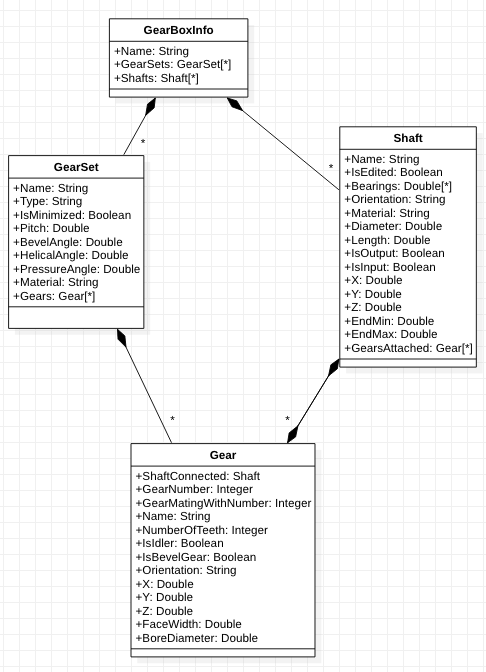
\includegraphics[scale=0.75]{uml}
    \caption{UML class diagram.}
    \label{fig:uml}
\end{figure}

\subsection{Windows}
Each window and page (a ``page'' in WPF is a section of a window that contains its own controls) of the application has its own XAML/C\# file as well as certain actions that the page does, such as window navigation or calling the backend model layer functions. The main window of the application (the window on which the user spends most of their time) is called \texttt{MainWindow}. From here, the user can access all other windows and pages of the application.

Since WPF is event-based (the system reacts and responds to user events), most of the logic in these windows is provided by the event handlers. An event handler is a function that is called by the system whenever a specific event is triggered. For example, when a button \texttt{Button1} is clicked, the method \texttt{Button1\_Click} is called. Every interactive element of the user interface has an event handler. The most common event is when a button is clicked, but there are other events that can be handled, such as when a user is typing into a text box.

\subsection{SolidWorks Macro}
The primary use of the application is to enter data for gear trains and have them be generated in SolidWorks. Using the SolidWorks API, this data can be sent to an existing SolidWorks process to be generated. The class \texttt{SolidWorksMacro}, which is used for sending a \texttt{GearBoxInfo} object to SolidWorks is being reused from the previous gear box system. This class did not need to be changed to work with our application, as the SolidWorks API has not changed.

The SolidWorks macro has its own definitions of the model classes (e.g. \texttt{Gear} in our model layer is equivalent to \texttt{Gear\_info} in the SolidWorks macro). When the button ``Generate in SolidWorks'' is pressed on the main window, the model classes are converted into SolidWorks macro classes. After this, the macro can call the SolidWorks API functions to have the gearbox generated in SolidWorks.

\subsection{Project File Structure}

In order to keep all code organized, a file system was designed which allows files to be organized and found much easier. Additionally, this helps us implement the MVVM architecture since each part of the application can be separated more easily. In the old gear design system (\cite{holman_automated_2018}), the interface and backend code were defined in the same files. The entire codebase for that system was only four files (each Windows Form window is divided into two or three files, here we are considering them to be as one file). Some of these files are thousands of lines of code long. Finding any code in a system like this is extremely difficult. Our project's file system is described in Table~\ref{tab:file_structure}.

\begin{table}[htb]
    \centering
    \caption{Project file structure.}
    \label{tab:file_structure}
    \begin{tabularx}{\textwidth}{||Y|Y|Y||}
        \hline Folder Name & Purpose & Example Files Contained Within \\ \hline \hline
        3rd & 3rd party libraries (including SolidWorks API) & SldWorks.dll \\ \hline
        Resources & Resources of the project (e.g., icons) & gear\_v11.ico \\ \hline
        Controls & Gearbox property control windows & GearPropControl.xaml.cs \\ \hline
        Helpers & Many helper classes and methods & UnitConverters.cs \\ \hline
        Models & MVVM model classes (no gear objects) & GearBoxSettings.cs \\ \hline
        SolidWorks & MVVM model classes (gear objects), SolidWorksMacro & Gear.cs \\ \hline
        Templates & Gear template files for SolidWorks & Parametric Spur Template.SLDPRT \\ \hline
        Views & The different pages/windows of the application & EditGearSetView.xaml \\ \hline
    \end{tabularx}
\end{table}

In addition to these project subfolders, there are some files in the root directory of the project. Most of these are default files required by WPF that we will never modify. The one notable file is MainWindow.xaml (and MainWindow.xaml.cs) which is the main window of the project. This is in the root folder (and not the Views folder) because it is the most important file of the project so it makes sense to put it in the project root.

\subsection{Application Flow}
With all parts of the application in place, including the model and system architecture, the application flow can be constructed. This is a way of visualizing the different actions the user can take, the system's response to them, and the next steps for the user and system. Figure~\ref{fig:func_dia} shows this in detail. This functional diagram was modified from the old gear design software (\cite{holman_automated_2018}).

The system exists as a mostly ``modeless'' design, meaning most user actions are available at all times (not dependent on system state). In Figure~\ref{fig:func_dia}, the large box in the middle represents the main window of the application, where the user has many actions they can perform, regardless of system state. However, certain actions would not work as desired if the system state is not correct (e.g. ``Generate in Solidworks'' will not generate anything if there are no gear sets). 

\begin{figure}[htbp]
    \centering
    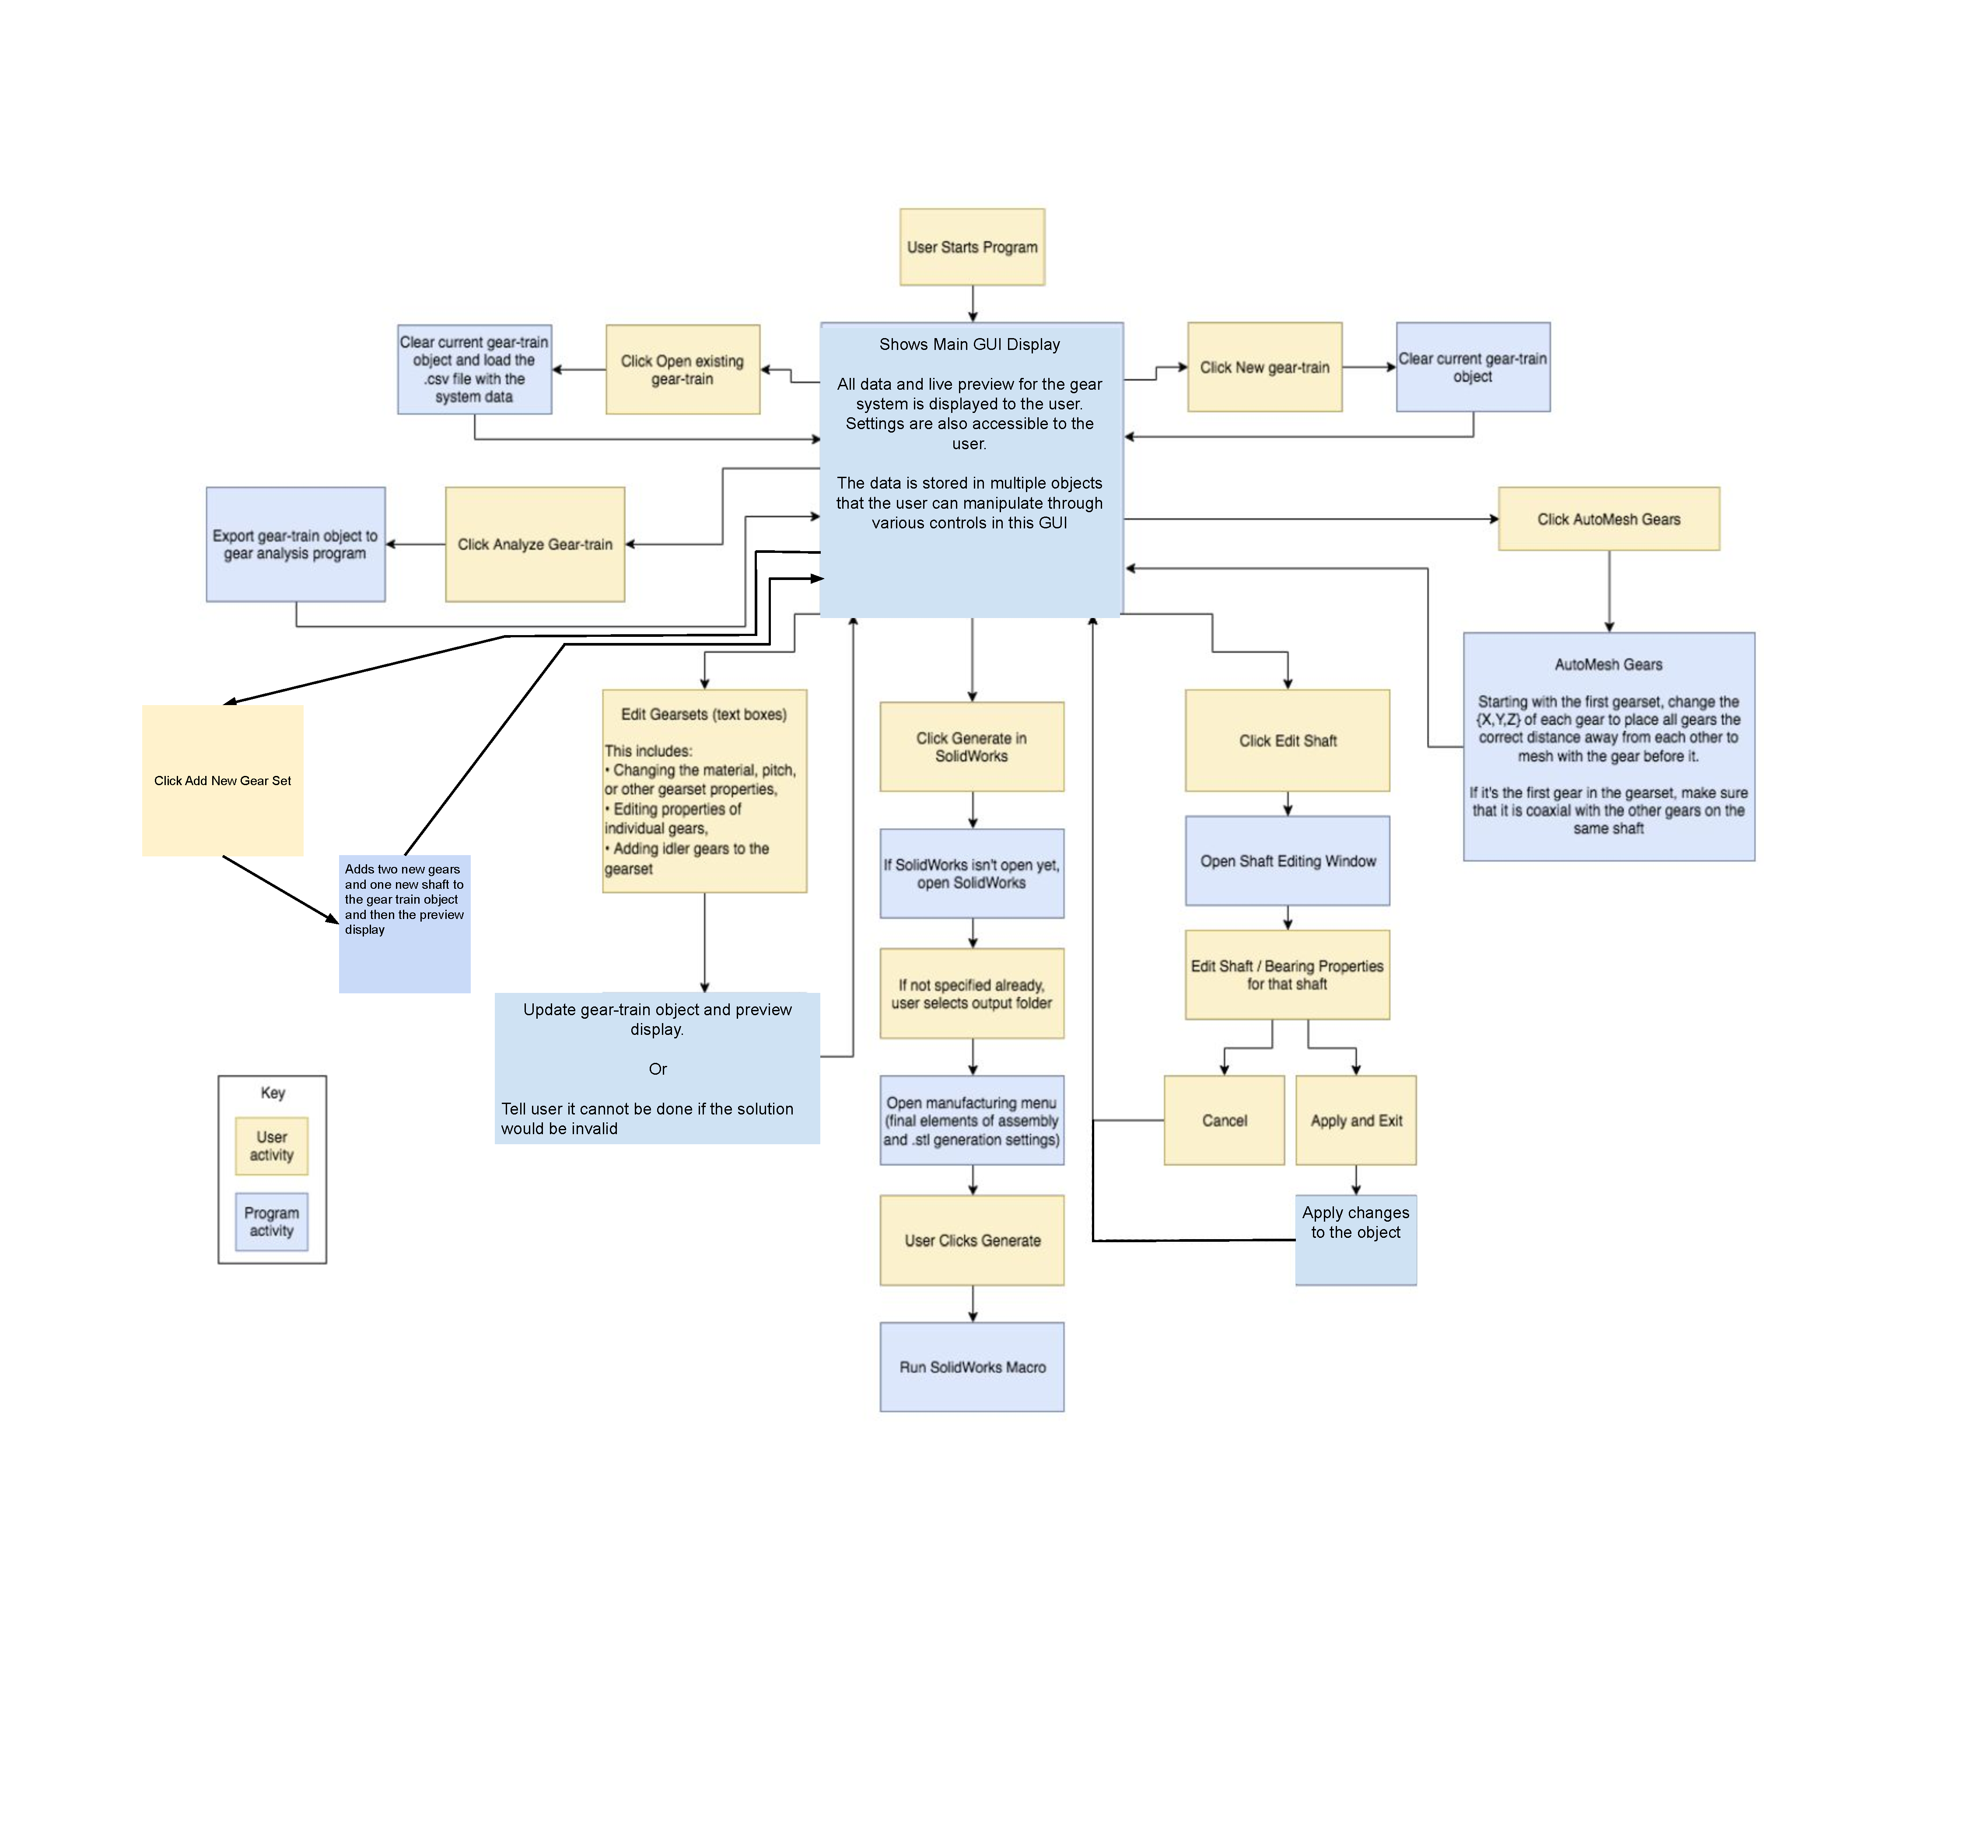
\includegraphics[angle=90,scale=0.36]{func_dia}
    \caption{Functional diagram showing user and system actions.}
    \label{fig:func_dia}
\end{figure}

\end{doublespace}